% REMEMBER: You must not plagiarise anything in your report. Be extremely careful.

\documentclass{l4proj}

    
%
% put any additional packages here
%
\usepackage{listings-rust}
\lstset{language=Rust, style=colouredRust}

\begin{document}

%==============================================================================
%% METADATA
\title{The IETF Transport Service API}
\author{Stuart Reilly}
\date{\today}

\maketitle

%==============================================================================
%% ABSTRACT
\begin{abstract}
    Network programming has been build around the Berkeley Sockets API since its inception in 1983.
    While the simplicity of this API, which abstracted file I/O and network I/O to a similar interface,
    is a testament to its longevity, modern network programming has changed in a manner which requires
    amounts of boilerplate code.
    This projects aims to investigate the possibility of a high-level API which removes the boilerplate
    associated with Berkeley sockets, and provide a protocol-agnostic, asynchronous API to application developers.
\end{abstract}

%==============================================================================

% EDUCATION REUSE CONSENT FORM
% If you consent to your project being shown to future students for educational purposes
% then insert your name and the date below to  sign the education use form that appears in the front of the document. 
% You must explicitly give consent if you wish to do so.
% If you sign, your project may be included in the Hall of Fame if it scores particularly highly.
%
% Please note that you are under no obligation to sign 
% this declaration, but doing so would help future students.
%
\newcommand{\consentname}{Stuart Reilly} % your full name
\newcommand{\consentdate}{\today} % the date you agree
%
\educationalconsent


%==============================================================================
\tableofcontents

%==============================================================================
%% Notes on formatting
%==============================================================================
% The first page, abstract and table of contents are numbered using Roman numerals and are not
% included in the page count. 
%
% From now on pages are numbered
% using Arabic numerals. Therefore, immediately after the first call to \chapter we need the call
% \pagenumbering{arabic} and this should be called once only in the document. 
%
% Do not alter the bibliography style.
%
% The first Chapter should then be on page 1. You are allowed 40 pages for a 40 credit project and 30 pages for a 
% 20 credit report. This includes everything numbered in Arabic numerals (excluding front matter) up
% to but excluding the appendices and bibliography.
%
% You must not alter text size (it is currently 10pt) or alter margins or spacing.
%
%
%==================================================================================================================================
%
% IMPORTANT
% The chapter headings here are **suggestions**. You don't have to follow this model if
% it doesn't fit your project. Every project should have an introduction and conclusion,
% however. 
%
%==================================================================================================================================
\chapter{Introduction}\label{ch:introduction}

% reset page numbering. Don't remove this!
\pagenumbering{arabic}

The Berkeley socket API (BSD sockets) allows an application to communicate over the Internet since 1983.
A key reason for its longevity is how a network socket is treated in the same way as a local file, once the socket has
been created.
This allows a programmer with understanding of local file I/O to work with network sockets.
While this model of network I/O has some similarities to local file I/O, in reality they are distinct and should be
treated as such.
One prime example of this is how network I/O has a range of protocols which can be used at each layer of the networking
stack, each providing different grantees and properties, and the application must specify which protocol stack to use.
Whereas in file I/O, there exists a protocol stack (file systems, storage interface, etc), but the application does not
need to manipulate the stack, as each protocol is a platform-specific way to handle the same operations.

Since BSD sockets required applications to decide the protocol stack, changing protocols would require the application
to be modified.
This may have contributed to the slow adoption of IPv6, since every application would have to be rewritten to use IPv6
rather than only the network implementation.
BSD sockets defined the default protocol to handle streams and datagrams are TCP and UDP, respectively.
While this may have aided in the adoption of these protocols and the growth of the Internet, it also hindered the
development of alternative protocols such as DCCP and SCTP .

Furthermore, BSD sockets exposes a synchronous API, providing blocking I/O .
Modern programming practices have changed to encourage the use of non-blocking I/O through the use of an asynchronous
API .
An asynchronous API allows the application to pass scheduling I/O calls to the implementation, often providing better
performance.

To resolve the above issues, a new networking API must be created.
Such an API must be protocol-agnostic and asynchronous, while allowing not reducing the possible uses of the API in
comparison to BSD sockets.
By being protocol-agnostic, the API decouples applications from the transport-layer, allowing new protocols to be
designed and used without applications having to be modified.
Modern network programming relies on asynchronous networking, which previously would require boilerplate over BSD
sockets.
By having the API be asynchronous, this boilerplate can be removed.

The aim of this project is to create an API which fulfills these requirements, and evaluate it in comparison to BSD
sockets.
The IETF Transport Services API will provide the overall design of the API, and Rust will be the implementation language
used.
Rust provides high-level safety with low-level performance and access, while also having be designed with concurrent
programming in mind.


%Why should the reader care about what are you doing and what are you actually doing?
%\section{Guidance}
%
%\textbf{Motivate} first, then state the general problem clearly.
%
%\section{Writing guidance}
%\subsection{Who is the reader?}
%
%This is the key question for any writing. Your reader:
%
%\begin{itemize}
%    \item
%    is a trained computer scientist: \emph{don't explain basics}.
%    \item
%    has limited time: \emph{keep on topic}.
%    \item
%    has no idea why anyone would want to do this: \emph{motivate clearly}
%    \item
%    might not know \emph{anything} about your project in particular:
%    \emph{explain your project}.
%    \item
%    but might know precise details and check them: \emph{be precise and
%    strive for accuracy.}
%    \item
%    doesn't know or care about you: \emph{personal discussions are
%    irrelevant}.
%\end{itemize}
%
%Remember, you will be marked by your supervisor and one or more members
%of staff. You might also have your project read by a prize-awarding
%committee or possibly a future employer. Bear that in mind.

%\subsection{References and style guides}
%There are many style guides on good English writing. You don't need to
%read these, but they will improve how you write.

%\begin{itemize}
    %\item
    %\emph{How to write a great research paper} \cite{Pey17} (\textbf{recommended}, even though you aren't writing a research paper)
    %\item
    %\emph{How to Write with Style} \cite{Von80}. Short and easy to read. Available online.
    %\item
    %\emph{Style: The Basics of Clarity and Grace} \cite{Wil09} A very popular modern English style guide.
    %\item
    %\emph{Politics and the English Language} \cite{Orw68}  A famous essay on effective, clear writing in English.
    %\item
    %\emph{The Elements of Style} \cite{StrWhi07} Outdated, and American, but a classic.
    %\item
    %\emph{The Sense of Style} \cite{Pin15} Excellent, though quite in-depth.
%\end{itemize}

%\subsubsection{Citation styles}

%\begin{itemize}
%\item If you are referring to a reference as a noun, then cite it as: ``\citet{Orw68} discusses the role of language in political thought.''
%\item If you are referring implicitly to references, use: ``There are many good books on writing \citep{Orw68, Wil09, Pin15}.''
%\end{itemize}

%There is a complete guide on good citation practice by Peter Coxhead available here: \url{http://www.cs.bham.ac.uk/~pxc/refs/index.html}.
%If you are unsure about how to cite online sources, please see this guide: \url{https://student.unsw.edu.au/how-do-i-cite-electronic-sources}.
%
%\subsection{Plagiarism warning}
%
%\begin{highlight_title}{WARNING}
%
%    If you include material from other sources without full and correct attribution, you are commiting plagiarism. The penalties for plagiarism are severe.
%    Quote any included text and cite it correctly. Cite all images, figures, etc. clearly in the caption of the figure.
%\end{highlight_title}
%

%==================================================================================================================================
\chapter{Background}\label{ch:background}
In this chapter, we research a suitable implementation language and existing attempts to replace the BSD Sockets API .

\section{Rust}\label{sec:rust}
Rust is a modern systems programming language, which aids developers “write faster, more reliable software”, according
to the Rust book (\cite{kalbnik_rustprogramminglanguage_}).
Rust targets systems level programming, similar to C and C++, but provides much greater safety in comparison.

One major issue with writing system software is ownership.
Who owns a resource, such as memory or file handles, and for how long.
In higher level languages, a garbage collector will ensure no resources live longer than they are needed, often through
the use of reference counting.
Garbage collection does elevate the burden of resource management from the developer, but in return, the developer has
much less control over resources, and the resources will live of a non-deterministic length of time with most garbage
collectors.
Languages like C and C++ require the programmer to manage resources, releasing them manually, leading to unreleased
resources if implemented incorrectly.
Rust enforces correct resource management by delegating all resource management to the compiler, through its borrow
checker.
Only a single entity can own a resource in Rust.
All other entities must use references to interact with the resource.
Furthermore, either a single mutable reference or an arbitrary number of immutable references can exist for a resource
at once.
These references cannot live longer than the entity owning the resource, which is enforced by the compiler.
When a reference goes out of scope, it is freed.
When an entity goes out of scope, there must be no remaining references to the entity, and the resources the entity owns
are freed.
Through this method, invalid references cannot exist, and it is impossible to release a resource which has already been
released.
A side effect of only allowing a single mutable reference, or an arbitrary number of immutable references, the compiler
can guarantee a compiled program is data race free.
This is because, only a single entity can modify a resource, while knowing no other entities can read the resource or
modify the resource.

Being a modern language, Rust provides some higher level concepts and construct to systems programming.
While Rust is a statically typed language, it provides local type inference, allowing for cleaning code.
Its type-system is inspired by other languages such as Haskell, as such a programmer can express a large amount of
information through the types they use alone.
Furthermore, Rust has support for higher-order functions, because functions are a first-class type.
Functions, such as map and fold, are provided, not directly for collections of items, rather iterators.
Iterators in Rust provide a functional method for working with collections of items, while providing performance similar
to a comparable loop construct.

Rust also emphasises its ability to provide “zero-cost abstractions”.
This means using high level constructs, such as iterators, do not inure any performance cost over using lower-level
constructs, allowing for code to be written faster and cleaner, without any performance impact.
Another example is Rust's Option type, which is either Some wrapping an object, or None.
This can be the equivalent to a \texttt{NULL}-pointer check in C, due to Rust's null-pointer optimisation, but is much
safer as the type-system forces the programmer to check for the presence of an object.
A Future in Rust is a type which is polled until it is complete.
A key feature of Rust's Futures is they only carry out work when polled, so there is no extra cost to use a Future.
Rather than polling all the Futures manually, a runtime is used to manage the Futures.
The runtime is responsible for distributing the Futures among its worker poll if applicable, and ensuring each Future is
polled.

Recently, Rust introduced support for \texttt{async/await} syntax~\citep{withoutboats_asyncawaitnotation_}.
A function can be marked as \texttt{async}, which changes the return type to be a \texttt{Future} wrapping the original
return type.
When an \texttt{async} function reaches an \texttt{await}, the poll being used to progress the Future returns Pending,
informing the runtime this \texttt{Future} is incomplete and another \texttt{Future} should be polled.
The \texttt{Future} will continue to return \texttt{Pending} until the \texttt{Future} being awaited completes,
at which point the function will continue until the next \texttt{await} or the function returns.
The new syntax allows for asynchronous code to be written quickly and cleanly with no runtime cost, compared too
manually handling \texttt{Future}s.

\section{BSD Sockets}\label{sec:bsd-sockets}
The Berkeley socket API (BSD Sockets) allows an application to communicate over the Internet since 1983.
A key reason for its longevity is how a network socket is treated in the same way as a local file, once the socket has
been created.
This allows a programmer with understanding of local file I/O to work with network sockets.
While this model of network I/O has some similarities to local file I/O, in reality they are distinct and should be
treated as such.
One prime example of this is how network I/O has a range of protocols which can be used at each layer of the networking
stack, each providing different grantees and properties, and the application must specify which protocol stack to use.
Whereas in file I/O, there exists a protocol stack (file systems, storage interface, etc), but the application does not
need to manipulate the stack, as each protocol is a platform-specific way to handle the same operations.

Since BSD Sockets required applications to decide the protocol stack, changing protocols would require the application
to be modified.
This may have contributed to the slow adoption of IPv6, since every application would have to be rewritten to use IPv6
rather than only the network implementation.
BSD Sockets defined the default protocol to handle streams and datagrams are
TCP\footnote{Transmission Control Protocol - IETF RFC793} and UDP\footnote{User Datagram Protocol - IETF RFC768},
respectively.
While this may have aided in the adoption of these protocols and the growth of the Internet, it also hindered the
development of alternative protocols such as DCCP\footnote{Datagram Congestion Control Protocol - IETF RFC4340} and
SCTP\footnote{Stream Control Transmission Protocol - IETF RFC4960}.

BSD Sockets primarily exposes a synchronous API, which does not match the nature of a network and does not reflect
modern network programming techniques.
While there is a non-blocking mode for BSD Sockets, it is error-prone and cumbersome to use effectively.
Furthermore, modern network programming utilises callbacks or futures, which BSD Sockets has no support for.
A custom event loop needs to be created and each socket needs to be polled by the application, rather than the API's
implementation.

\section{Post Sockets}\label{sec:post-sockets}
Post Sockets~\citep{kuhlewind_postsocketsabstract_} is an API intended to provide an asynchronous, message-orientated,
transport-protocol independent networking API to be used instead of BSD Sockets (Sockets).
\citet{kuhlewind_postsocketsabstract_} identified Sockets requires the user to tightly couple their program with a
specific transport-protocol.
This lead Post Sockets to be designed, so the user relies on a set of semantics, which could be upheld by an arbitrary
protocol, rather than a specific protocol.

As~\cite{kuhlewind_postsocketsabstract_} explains, modern networked devices have multiple interfaces, which would
provide natural support for multipath communications using protocols such as
MPTCP\footnote{Multipath TCP Extensions - IETF RFC6842}.
The existing sockets API provides limited support for multipath communications, whereas Post Sockets has explicit
support through its \emph{Configuration} object.
Post Socket's \emph{Configuration} objects allow the user to specify a collection of possible protocol stack
configurations.
This provides the user with explicit control over the possible protocol stacks used, and the options each stack has.

Rather than providing a byte-stream orientated API like sockets, Post Sockets exposes a message-orientated API .
Typed messages would be given to or received from a \emph{Carrier} (protocol stack-independent object which sends and
receives messages) as this allows both byte-stream and datagram oriented transport protocols to be supported.

Another point raised by~\cite{kuhlewind_postsocketsabstract_} is layering encryption over the existing sockets API .
Opening a TCP connection with
TLS\footnote{Transport Layer Security - IETF RFC8446} requires two handshakes to happen sequentially: the
transport-layer handshake and the encryption-layer handshake, which increases latency.
To avoid this Post Sockets defines an \emph{Association} object, which contains long-term state between a local endpoint
and a remote endpoint.
This can contain data such as pre-shared keys and cryptographic session resumption parameters.
New \emph{Carrier}s can be created from an existing \emph{Association} object, removing the need to repeat an
encryption-layer handshake between the same local endpoint and remote endpoint.

\section{NEAT}\label{sec:neat}
The NEAT API~\citep{khademi_neatplatformprotocolindependent_2017} is a library to provide a platform and protocol
agnostic network access.
\citet{khademi_neatplatformprotocolindependent_2017} identifies transport-layer protocols are implemented within the
operating system's kernel, and as such are bound by the release cycle of the kernel.
NEAT has been designed as a user-space library, rather then a kernel-space library like Sockets, to allow for new
transport-layer protocols to be included, irrespective of the kernel release cycle.

The duration of kernel release cycles is one of the reasons alternative transport layer protocols have limited uptake.
To add a new transport protocol to sockets, a new kernel release must be developed with this new protocol
NEAT is a user-space library, therefore supports both kernel-space and user-space transport protocols.
User-space transport protocols can be implemented and included in NEAT, independent of the kernel release cycle.
This removes the need to implement new transport protocols over UDP,
removing the often duplicated code to use UDP as a substrate for the protocol.

Existing network applications must specify the protocols they wish to use.
NEAT does not require the application to do this, rather NEAT determines a collection of suitable protocols internally
either from a set of allowed protocols from the user or from all supported protocols.
The method used to select the optimal protocol stack is called Happy Eyeballs~\citep{pauly_happyeyeballsversion_}.
This allows for alternative protocols, including user-space protocols, to be attempted while using traditional protocols
as fallbacks.

\section{TAPS}\label{sec:taps}
Transport Services~\citep{pauly_architecturetransportservices_2020} is proposed standard from the IETF TAPS working
group.
\citet{pauly_architecturetransportservices_2020} identified BSD Sockets did not allow sockets which conceptually
communicated the same data, could not make use of the same API calls.
For example, an encrypted TLS stream could not use the same \texttt{send()} and \texttt{recv()} calls as an unencrypted
TCP stream.
Therefore, TAPS was designed to provide a unified API for all connections which communicate the same data conceptually.

\begin{figure}
    \begin{verbatim}
    Pre-Establishment     :       Established             : Termination
    -----------------     :       -----------             : -----------
                          :                               :
+-- Local Endpoint        :           Message             :
+-- Remote Endpoint       :    Receive() |                :
+-- Transport Properties  :       Send() |                :
+-- Security Parameters   :              |                :
|                         :              |                :
|               InitiateWithSend()       |        Close() :
|   +---------------+   Initiate() +-----+------+ Abort() :
+---+ Preconnection |------------->| Connection |-----------> Closed
    +---------------+ Rendezvous() +------------+         :
   Listen() |             :           |     |             :
            |             :           |     v             :
            v             :           | Connection        :
    +----------+          :           |   Ready           :
    | Listener |----------------------+                   :
    +----------+  Connection Received                     :
                          :                               :
    \end{verbatim}
    \caption{Diagram to show the lifetime of a Connection object
            (Source:~\citet[fig:4]{pauly_architecturetransportservices_2020})}
    \label{fig:tapsConLife}
\end{figure}

TAPS is designed around the lifecycle of a \connection{} object, which is a representation of one or more transport
protocols that send and recieve data between a local and remote machine.
As shown in Figure~\ref{fig:tapsConLife}, a \connection{} object has three stages in its lifecycle: Pre-Establishment,
Established and Termination.

Pre-Establishment is the stage where the \connection{} is created, either directly via the \preconnection{} object's
\texttt{Initiate()}, \texttt{InitiateWithSend()} and \texttt{Rendezvous()} methods, or when a \listener{} receives a
\connection{}.
The \texttt{Initiate()} method is a traditional connection establishment between a local and remote,
\texttt{InitiateWithSend()} method allows data to be sent with the connection establishment
(0-RTT\footnote{Zero Round Trip Time}), and \texttt{Rendezvous()} is use to establish a peer-to-peer connection.
A \preconnection{} represents a potential \connection{}, containing the parameters of a possible future \connection{}.
It contains the definition of the local and/or remote machine via the Local or Remote Endpoints respectively, the
properties the underlying transport protocol must have, and optional security parameters.
A \listener{} object can be created from a \preconnection{} to listen for incoming \connection{}s which match the
properties the creating \preconnection{} has.

Established is the stage when the \connection{} sends and receives data.
\connection{}s communicate with strongly typed messages, rather than the raw bytes the underlying transport protocols
may use.
A \connection{} produces events for when a message been received and when data has been successfully sent, as well as
to signify errors have occurred.
These events are the mechanism TAPS uses to ensure it's API is asynchronous, but an implementation of TAPS does not have
to expose these events directly to the user.
The implementation is free to expose the asynchronous nature of the API is the method which idiomatic for the language,
such as futures or call backs.

Termination is the stage where the \connection{} is closed and cleaned up.
The user will call the \connection{}'s \texttt{close()} or \texttt{abort()} methods to gracefully or forceably end
the \connection{} and cleanup its resources.

No where in the TAPS API is the user able to specify the underlying transport protocol, Rather they specify the
properties the underlying transport protocol must uphold.
\citet[§~5.2]{trammell_abstractapplicationlayer_2020} has defined a set of properties underlying protocols can have,
and the preference a user can have for a property to be upheld.
The implementation of TAPS creates a list of transport protocols it supports, in order of most to least preferred,
excluding any supported protocols which either do not support a “Require” property or support a “Prohibit” property.
A transport protocol is deemed more preferred over another if it contains more “Prefer” properties and/or less “Avoid”
properties.

Since TAPS aims to provide a unified API for connections which communicate the same data, the same data must be able to
be sent/received on different transport protocols.
The two types of transport protocols are byte-stream orientated and datagram orientated.
Datagram orientated transport protocols have natural message boundaries as the boundaries of the datagrams, but
byte-stream orientated transport protocols lack this.
TAPS defines a \framer{} to define message boundaries for protocols which may or may not have natural message
boundaries.
A simple \framer{} could prepend each message with the length of the message, or define an end-of-message sequence for
example.

%What did other people do, and how is it relevant to what you want to do?
%\section{Guidance}
%\begin{itemize}
%    \item
%      Don't give a laundry list of references.
%    \item
%      Tie everything you say to your problem.
%    \item
%      Present an argument.
%    \item Think critically; weigh up the contribution of the background and put it in context.
%    \item
%      \textbf{Don't write a tutorial}; provide background and cite
%      references for further information.
%\end{itemize}

%==================================================================================================================================

\chapter{Analysis/Requirements}\label{ch:analysis/requirements}
The project will aim to produce a high-level, typed and asynchronous networking API, based on the IETF's TAPS, in the
Rust programming language, making use of Rust's \asyncawait syntax and \texttt{Future}s.
This API is intended to be a replacement for BSD sockets, and as such will provide similar functionality, albeit at a
higher level.
Since the project will be based on TAPS, \preconnection{}, \framer{}, \listener{} and \connection{} in this chapter
follow the definition discussed in Section~\ref{sec:taps}, to be fully defined in Section~\ref{sec:abstract-api}.

In this chapter we define a set of functional and non-functional requirements, splitting each into ''required'' and
''optional''.
These requirements must fulfill the aims outlined in Chapter~\ref{ch:introduction} and are intended to be built upon and
make use of the prior research discussed in Chapter~\ref{ch:background}.

\section{Functional Requirements}\label{sec:functional-requirements}

\subsection{Required}\label{subsec:required}
The \preconnection{} must allow for the user to specify both the local and remote machine the resulting \connection{}
will operate with.
Without this functionality, a \connection{} would not be able to be established as there would be nothing to establish
between.

The API must provide enough functionality to support a single-client and single-server example.
This is required, because this is a minimum requirement to be able to be a basic replacement for BSD sockets.
Furthermore, most network communication occur this style, and the remaining can be recreated using this style.
As such a \preconnection{} must be defined which can initiate a \connection{} object, or begin listening for
\connection{}s.

The API must be asynchronous, utilising futures as the mechanism of handling asynchronous events.
This is required, because one the main issues with BSD sockets discussed in Chapter~\ref{ch:background} was its
synchronous nature.
Asynchronous network programming is the modern technique, as such must be the primary method of using a new networking
API .
Futures are the de-facto standard method for asynchronous programming in Rust, as such they shall be used.

The API must define a \connection{} object which can send and receive typed data.
As discussed in Chapter~\ref{ch:background}, one of the issues with BSD sockets is they only support sending byte
streams or byte datagrams for TCP and UDP sockets respectively.
As such the API must expose a mechanism for typed data to be passed to a \connection{} object, which will converted into
the appropriate byte structure by the \connection{} object.

The API must define a mechanism to frame messages of a known size.
This is required, because in order to transform underlying transport layer data to and from useful message data,
it must be framed.
Without a framing mechanism, a byte-stream based transport layer will not be able to send and received typed data,
which is required by the previous requirement.

\subsection{Optional}\label{subsec:optional}

The API could provide a mechanism to frame messages of an unknown size.
This would allow byte-stream based transport layer data to be transformed to and from useful message data, even without
knowing the size of the data being transferred.
Since this section of the TAPS specification is not well-defined and is under continuous modification, this will not be
required to be implemented by this project.

The API could provide a \connection{} object which can receive partial data.
Since the underlying transport layer could not provide reliable data transfer, the \connection{} object could provide
partial data, which could be completed with subsequent packets.
Since this section of the TAPS specification is currently not well-defined and is under continuous modification, this
will not be required to be implemented by this project.

The API could provide a mechanism to enforce \preconnection{} object validity at compile-time through the use of Rust's
type system.
A \preconnection{} requires a remote endpoint or local endpoint to initiate a \connection{} or begin listening for
\connection{}s, respectively.
This can be implemented through a runtime error trivially, but to ensure the API is as safe as possible, this could be
implemented as a compile-time error.
Since implementing this as a compile-time error is non-trivial, and does not impact the usability of the API, this will
not be required to implement this project.

\section{Non-Functional Requirements}\label{sec:non-functional-requirements}

\subsection{Required}\label{subsec:required2}

The API must expose a “self-documenting” API, meaning the names of methods, method arguments, objects and constants must be
meaningful and describe their use.
This ensures the API describes how to use itself through its naming, using explicit documentation to augment this description.
Furthermore, this lowers to learning curve of the API, possibly increasing rate of adoption.

The API must allow users of the API to provide their own types for sending and receiving over a \connection{}.
Without this mechanism, the API will be very restrictive and not useful.
The Rust ecosystem has support for arbitrary type serialisation and deserialisation through the Serde library, as such this
will likely be used to provide this mechanism.

\subsection{Optional}\label{subsec:optional2}

The API should not have a large impact performance over raw BSD sockets.
A large performance impact will hinder the adoption of the API, and as such should be avoided.
Since this is primarily a proof-of-concept project, this is not required, but should still be taken into account.

%==================================================================================================================================

\chapter{Design}\label{ch:design}
In this section, we discuss the high level design of the API, without implementation specific details.
First, a short discussion on the abstract nature of the API .
Followed by the overall flow of the API will be discussed and how each of the main objects connect together.
Then, each of the main objects in the API will be discussed in the order of the rough flow of the API, discussing
the design decisions made for each object.

\section{Flow}\label{sec:flow}
\begin{figure}[h]
    \centering
    \includegraphics[width=\textwidth]{diagrams/flow}
    \caption{A diagram to show how the three main objects flow from one to another.
    Oval nodes are objects, rectangular nodes are states in the transition between objects, dashed arrows are
    asynchronous state changes, and solid arrows are synchronous state changes.}
    \label{fig:flow}
\end{figure}

\begin{figure}[h]
    \centering
    \includegraphics[width=\textwidth]{diagrams/lidecycle.png}
    \caption{A diagram to show a high-level view of the actions that occur during the lifecycle of a Connection object.
    Method calls in italics are internal calls.}
    \label{fig:lifecycle}
\end{figure}

As shown in Figure~\ref{fig:flow}, there are both asynchronous and synchronous sections of opening a \connection{}.
The asynchronous sections are when the program would have to carry out some I/O, for example binding a \listener{}
to a port, or establishing a \connection{} to a remote device.
The remaining sections are either a trivial object creation or solving properties, as such are synchronous.
Solving properties can contain a concurrent implementation if the implementation deems this necessary.
Figure~\ref{fig:lifecycle} shows the lifecycle of a \connection{} object.
All \connection{} objects are created either directly via \texttt{initiate()} or indirectly via a \listener{}.
A \connection{} then communicates with the network through a \framer{}, until \connection{} is no longer
needed and \texttt{close()} or \texttt{abort()} are called.
Rust's \texttt{Drop} allows the user of the API to not call either \texttt{close()} or \texttt{abort()} explicitly, as
it allows arbitrary code to be executed when a variable goes out of scope.
Since utilising \texttt{Drop} does not allow for errors to be propagated back to the user, it will likely be similar to
a \texttt{close()} call where all errors are discarded.
Section~\ref{subsec:connection} describes the difference between \texttt{close()} and \texttt{abort()}.
See Section~\ref{subsec:framer} for details on why a \framer{} is required for a \connection{}.

\section{Abstract API}\label{sec:abstract-api}
The API will be expressed primarily through abstract types with multiple possible concrete implementations.
Users of the API will operate almost exclusively with the traits (abstract types) in order to allow the underlying
implementation and protocol stack to change with minimal impact to the user's code.
If the API was defined with concrete types through the use of structs, the underlying implementation which handles
the native network would not be able to impact without major changes to the user's code.
Due to Rust's heavy use of monomorphisation and lack of runtime generics, the traits will be used through trait objects
to allow the API to be dynamically linked.
Trait objects are Rust's method of dynamic dispatch and pseudo runtime generics.
All trait objects must be wrapped in \texttt{Box} and marked as \texttt{dyn}, for example
\texttt{Box<dyn Connection<F>>}, which leads to cluttered code.
This can be mediated through type alias, so for example if \texttt{type ConnectionObj<F> = Box<dyn Connection<F>>;} was
defined, \texttt{ConnectionObj<F>} can be used instead.
While using trait objects would add a performance overhead due to pointer indirection and dynamic dispatch, the benefit
of dynamic linking and alternative distribution out ways this.

\subsection{Preconnection}\label{subsec:preconnection}
First the user will create a \preconnection{}, which will be used to define the properties a \connection or \listener
must have.
A \preconnection{} object is a configuration object.
It contains the endpoints, both local and remote, a \connection{} or \listener{} should connect or bind too
respectively, as well as the properties the resultant \connection{} or \listener{} should have.
\cite[§~5.2]{trammell_abstractapplicationlayer_2020} defines a set of properties a \preconnection{} can configure.

\begin{lstlisting}[float=h, label=lst:preconnection, caption={The Preconnection struct, showing the four
generic parameters.}]
pub struct Preconnection<F, L, R, I=DefaultImpl>
where
    F: Framer,
    L: EndpointState,
    R: EndpointState,
    I: Implementation
{
    local: L,
    remote: R,
    framer: F,
    trans: TransportProperties,
}
\end{lstlisting}

The \preconnection{} type will be defined as a concrete struct, rather than a trait, unlike the \listener{} and
\connection{} types.
Since a \preconnection{} is a configuration type which is independent of the underlying implementation, using a
trait would be redundant as each underlying implementation would implement the trait identically.
Furthermore, due to issues with the Rust compiler, it is difficult to change generic parameters with trait methods,
which is used to ensure endpoints are specified at compile time.
Listing~\ref{lst:preconnection} shows the definition for the \preconnection{} struct and the generic parameters it
has.
The generic parameters L and R are used to represent the possible local and remote endpoints respectively.
See Section~\ref{sec:preconnection-endpoint-safety} for details on these parameters.

\subsection{Implementation}\label{subsec:implementation}
While the user should not focus on the underlying implementation of the traits, it needs to be defined for the
\preconnection{} to know how to instantiate them.
The \emph{Implementation} trait is a primarily an internal trait as it specifies the underlying implementation, but is
public to allow the end user to select from multiple implementations, and create custom implementations.
The specific implementation will be specified with \preconnection{}'s \texttt{I} generic parameter, which implements the
\emph{Implementation} trait.

\begin{lstlisting}[float=h, label=lst:impl, caption={The Implementation trait.}]
pub trait Implementation {
    async fn connection<F, L, R>(
        framer: F,
        local: Option<L>,
        remote: R,
        props: &TransportProperties,
    ) -> Result<Box<dyn Connection<F>>, Error>
    where
        F: Framer + Clone,
        L: Endpoint,
        R: Endpoint;

    async fn listener<F, L, R>(
        framer: F,
        local: L,
        remote: Option<R>,
        props: &TransportProperties,
    ) -> Result<Box<dyn Listener<F, Item = Result<Box<dyn Connection<F>>, Error>>>, Error>
    where
        F: Framer,
        L: Endpoint,
        R: Endpoint;
}
\end{lstlisting}

One method to utilise the \emph{Implementation} is to have the methods take either \texttt{\&mut self} or
\texttt{\&self}, which are a mutable reference to the object and an immutable reference to the object respectively
(similar to \texttt{this} in C++), and pass the implementation as a parameter when constructing a \preconnection{}.
This would require the end user to always specify an implementation when constructing a \preconnection{}, even when
using the default implementation.
See Listing~\ref{lst:preconnBad} for an example of this method.

\begin{lstlisting}[float=h, label=lst:preconnBad, caption={An example of how to construct a
Preconnection if the Implementation trait is to be passed when the Preconnection is constructed}]
fn example() {
    let preconnection = Preconnection::new(Tokio, TransportProperties::default(), ...);
    ...
}
\end{lstlisting}

An alternative method is to have the \emph{Implementation} methods not take \texttt{self} in any form.
This would allow the \preconnection{} to specify a default implementation using Rust's default generic parameter
mechanism.
See Listing~\ref{lst:preconnGood} for two examples of this method, the first \preconnection{} is an example of using
the default implementation, and the second \preconnection{} shows how a custom implementation would be specified.
Since the underlying implementation is not intended to be a focus for the user, this method will be used.

\begin{lstlisting}[float=h, label=lst:preconnGood, caption={An example of how to construct a
Preconnection if the Implementation trait is used as a marker.}]
fn example() {
    let preconnection = Preconnection::new(TransportProperties::default(), ...);
    let custom_impl_preconn = Preconnection::<_,_,_,Tokio>::new(TransportProperties::default(), ...);
    ...
}
\end{lstlisting}

\subsection{Endpoint}\label{subsec:endpoint}
A \connection{} and \listener{} need to know what to connect to or listen to respectively, and this is specified in the
creating \preconnection{} by giving it either local or remote \Endpoint{}s.
An \Endpoint{} is a type which represents possibilities, either a local or remote endpoint.
This could be a string containing a domain name, or an IPv6 address and port number for example.
It does not represent an endpoint, rather a possible endpoint which needs to be resolved into a \texttt{SocketAddr}.

\begin{lstlisting}[float=h, label=lst:endpoint, caption={The Endpoint Trait with the resolve method returning an
        Iterator.}]
pub trait Endpoint: Send + 'static {
    type Error: Send + Error;
    type Iter: Iterator<Item = SocketAddr> + Send;

    async fn resolve(self) -> Result<Self::Iter, Self::Error>;
}
\end{lstlisting}

As shown in Listing~\ref{lst:endpoint}, \Endpoint{} requires a \texttt{resolve} method.
This method is where a possible endpoint is resolved into a \texttt{SocketAddr}.
There are no implementations of the trait provided as Rust does not allow a trait to be implemented twice for the same
type.
A trivial implementation could be provided for the \texttt{SocketAddr}, but implementations with traits similar to
Rust's \texttt{ToSocketAddrs} trait, which have implementations for \texttt{SocketAddr}, cannot be used as a blanket
implementation for \Endpoint{}.
All implementations of \Endpoint{} must also be \texttt{Send} since \texttt{resolve} is async, which means it will
make use of a \texttt{Future}, which could be run on a different thread.
The associated types \texttt{Error} and \texttt{Iter} require the type to be of type \texttt{Send} for the same reason.
Furthermore, since there is no guarantee as to how long the \texttt{Future} will take to complete, the type which
implements \Endpoint{} must exist for the length of the program, hence must have a \texttt{'static} lifetime.
Upon a successful resolution, the resolved \texttt{SocketAddr}s are returned as an \texttt{Iterator}.
Initially \texttt{resolve} returned a \texttt{Vec<SocketAddr>}, primarily because it allowed for simpler type
definitions and didn't require an associated type.
Using a \texttt{Vec} requires explicit allocation, which would lead to an unnecessary performance hit when an
implementation operates on an \texttt{Iterator} internally or is a trivial implementation such as for
\texttt{SocketAddr}.
As such, \texttt{resolve} was modified to return an \texttt{Iterator}, which was defined as the associated type
\texttt{Iter}.
This can lead to a long type definition for \texttt{Iter}, but this can be mediated with the unstable feature
\texttt{type\_alias\_impl\_trait}\footnote{\url{https://github.com/rust-lang/rust/issues/63063}}.

\subsection{Connection}\label{subsec:connection}
Once the \preconnection{} is fully configured, it's \texttt{initiate()} method can be called to initiate connection
establishment to the \preconnection{}s remote \Endpoint{}.
A \connection{} object represents a messaged-orientated connection between a local and remote endpoint.
It wraps an underlying protocol stack the user of the API specifies with the \emph{Implementation}
parameter of the \preconnection{} which created the \connection{}.
The user shouldn't need to focus on the underlying protocol stack as the \texttt{initiate()} method and
\listener{} will ensure the required properties for the \connection{} are upheld.
A \connection{} cannot be created without a remote endpoint.
Without a remote endpoint, a \connection{} has nothing to connect to.
The remote endpoint can either be given to the creating \preconnection{} for use in the \texttt{initiate()} method,
or taken from the incoming \emph{connection} a \listener{} receives.
If the creating \preconnection{} is given a local endpoint, the \texttt{initaite()} method will ensure the resulting
\connection{} is between the required remote endpoint and given local endpoint.
By default, the \texttt{initiate()} method will attempt to establish a \emph{connection} between the required remote
endpoint and any applicable local endpoint.

\begin{lstlisting}[float=h, label=lst:connection, caption={The Connection trait.}]
pub trait Connection<F, S, R>
where
F: Framer<S, R>
{
    async fn send(&mut self, data: S) -> Result<(), Self::Error>
    where
        S: Encode;

    async fn receive(&mut self) -> Result<R, Self::Error>
    where
        R: Decode;

    async fn close(self: Box<Self>) -> Result<(), Self::Error>;

    fn abort(self: Box<Self>);
}
\end{lstlisting}

The \connection{} will be defined as a trait, and will be constructed with the \preconnection{} object's
initiate method.
Each implementation of the \emph{Implementation} trait will have its own underlying representation of a connection
between a local and remote endpoint.
Defining a \connection{} as a trait allows the user's code to use any underlying representation of a connection
without having to specifically handle each possible representation.
As shown in Listing~\ref{lst:connection}, the \texttt{close()} and \texttt{abort()} methods take \texttt{Box<Self>}
rather than \texttt{Self}.
Since \connection{} is to be a trait object, it must be object safe.
An object safe trait, must not require implementations to be sized, not have any methods which consume \texttt{Self}, no
associated constants and all supertraits must be object safe.
As such, for the close and abort methods cannot take \texttt{Self}, instead take \texttt{Box<Self>} since it is sized
and does not require \texttt{Self} to be sized.
These methods consume \texttt{Box<Self>} because the Rust compiler can ensure no other variable has ownership of the
\connection{} when it is closed or aborted, preventing the \connection{} from be used after its closed or aborted.

Both \texttt{close()} and \texttt{abort()} methods are provided because a \texttt{close()} will gracefully close the
underlying connection.
For connection-oriented transport protocols, \texttt{close()} should inform the remote endpoint the connection
is closed, allowing for resource cleanup.
Connectionless transport protocols may inform the remote endpoint if applicable.
On other the other hand, \texttt{abort()} should clean up the local resources, but it makes no guarantee about whether
or not the remote endpoint is informed of the connection closing.
If a \connection{} has a \texttt{Drop} implementation, it should have similar semantics to \texttt{close()}, but
discard errors produced.

\subsection{Listener}\label{subsec:listener}
Once the \preconnection{} is fully configured, it's \texttt{listen()} method can be called to bind a \listener{} to the
\preconnection{}'s local \Endpoint{}.
A \listener{} represents a stream of incoming \connection{}s for a local endpoint.
It is bound to the local endpoint in the creating \preconnection{}, and listens for incoming \connection{}s,
represented as an asynchronous stream of \emph{Connections}.
A \listener{} cannot be created without a local endpoint.
Without a local endpoint, the \listener{} cannot be bound and cannot listen for incoming \connection{}s.
The local endpoint must be given to the creating \preconnection{} for use in the \texttt{listen()} method.
A remote endpoint is optional, and if it is given to the creating \preconnection{}, the resulting \listener{} will only
accept \connection{}s from the given remote endpoint.
A \listener{} created without a remote endpoint will accept any incoming \connection{}s.

\begin{lstlisting}[float=h, label=lst:listener, caption={The Listener trait, showing the Stream
implementation requirement for all implementers.}]
pub trait Listener<F, S, R>: Stream<Item = Result<Box<dyn Connection<F, S, R>>, Error>>
where
    F: Framer + Clone,
{
    fn connection_limit(&mut self, limit: usize);
}

\end{lstlisting}
One approach to design this trait is to define the trait with a method which returns a \texttt{Future} that resolves
into a Connection when one is received.
An issue with this design is it does not a true reflection of the \listener{} interface.
Conceptually a \listener{} is an asynchronous stream of \connection{}s, and this design represents a
\listener{} as an object which is idle until the user requests a \connection{}.
At this point it then begins to listen for incoming connections, which could lead to lost connections.
A better design is to have all implementations of the \listener{} trait also implement the \texttt{Stream} trait
from the futures crate.
This allows a \listener{} to make use of the existing \texttt{Stream} ecosystem, such as the \texttt{StreamExt}
trait, which provides an \texttt{Iterator}-style interface to a \texttt{Stream}.
As shown in Listing~\ref{lst:listener}, the implementation for the \texttt{Stream} trait is required to produce an Item
which is either a \connection{} or an \emph{Error}.
For a \framer{} to be given to a \listener{}, a new version of it needs to be given to each \connection{}
received.
As such, \framer{}'s which can be used with the \listener{} trait must implement \texttt{Clone}.

The \connection{} and \listener{} traits and the \preconnection{} struct will be generic over the framer
used to frame the data which the connections will be operating on.
This will ensure the \connection{}s can only handle specific strongly-typed data.
All methods on the \connection{} trait which either receive data or send data will utilise this generic parameter in
their return value and parameters respectively.
The \preconnection{}'s listen and initiate methods will pass this generic parameter to the new \listener{}
object or \connection{} object respectively.
An alternative approach is to have the traits generic over the data which the \connection{}s will be operating on.
The issue with this approach is the compiler cannot ensure a \connection{} has certain properties which methods
could rely on.
For example, a method could require a \connection{} which is framed with TLS .
If the \connection{} is generic over the \framer{}, the compiler can ensure only \connection{}s which are
framed with TLS are used, ensuring the data being transmitted is encrypted.
Furthermore, a collection of traits a \framer{} could implement could be created to ensure only \connection{}s
with \framer{}s which have specific properties can be used with certain methods.

\subsection{Framer}\label{subsec:framer}
When a \connection{}'s \texttt{send()} method is called, the message it's given is framed by the \connection{}'s
\framer{} before being passed to the underlying transport layer.
Similiarly, during a \connection{}'s \texttt{recv()} method, when data is received, the message is deframed from the
raw bytes by the \connection{}'s \framer{}.
\begin{lstlisting}[float=h, label=lst:framer, caption={The Framer trait, showing the Send and 'static
requirements for all implementers, and associated types.}]
pub trait Framer<S, R>: Send + Sync + 'static {
    type Input: Encode + Send;
    type Output: Decode;
    type MetaKey;
    type MetaValue;
    type Error: StdError + Send;

    fn frame(&mut self, item: Self::Input, dst: &mut BytesMut) -> Result<(), Self::Error>
    where
        S: Encode;

    fn deframe(&mut self, src: &mut BytesMut) -> Result<Self::Output, DeframeError<Self::Error>
    where
        R: Decode;

    fn add_metadata(&mut self, key: Self::MetaKey, value: Self::MetaValue);
}
\end{lstlisting}

A \framer{} trait defines a type which can frame and deframe a given piece of data, as well as optionally store
metadata for use in framing and deframing.
Datagram-orientated transport protocols like UDP have defined boundaries for messages, therefore don't require a method
of defining these boundaries.
Stream-orientated transport protocols like TCP do not have defined boundaries as they present a stream of bytes.
A \framer{} defines the message boundaries, for example prepending the message with the length of the message or
defining an end-of-message sequence.

The \framer{} must be generic over the data types it will frame and deframe.
By having a \framer{} be generic over both the data it can frame and deframe, different types can be used for input
and output, removing the chance of the end user using the incorrect data.
The Input and Output types are defined as associated types.
This allowed the implementation to specify the accepted types, rather than the end user, which allows an implementation to
restrict what data it can send and receive.
An alternative approach is to defined Input an Output as generic types on the \texttt{frame()} and \texttt{deframe()}
methods respectively.
This would allow the end user to pass an arbitrary type which implements a trait, which could be specified by the
implementation.
Such an approach would make it very difficult to work with header information.
For example, a HTTP framer would not be able to return the status code to the end user.
Associated types mean the implementation can limit the types the end user can use to type which handle such header data.
These types can contain their own generic parameters, for example a HTTPResponse object could have a generic type for
the body of the response, which can be restricted to types which implement \decode{}.
Listing~\ref{lst:framer} shows the Input and Output types as associated types.
The MetaKey and MetaValue types are associated types because they should not be specified by the end user.

All implementations of \framer{} must implement \texttt{Send} and \texttt{Sync}, as well the type definition having
a static lifetime.
\texttt{Send} and \texttt{Sync} are required to allow the \framer{} to be passed between threads and accessed from
different threads.
While a \texttt{Future} does not specify it will be executed on a different thread than it was created, but it allows
it so a \framer{} must be able to be passed to another thread.
Since \framer{}'s methods use \texttt{\&mut self}, a \framer{} may be accessed by a thread other than the thread
which created it, so a \framer{} must be able to be accessed from different threads.
\texttt{Future}s require that all types which are used within the \texttt{Future} must live longer than the
\texttt{Future}.
Rust allows type to be defined within functions, so the type definition would live for the duration of the function,
meaning the type cannot be referenced outside the function.
Since a \texttt{Future} can take an indeterminate length of time to complete, all \framer{} type definitions must
have a static lifetime, which means it lives for the lifetime of the program.

An example is a HTTP framer, which can frame a HttpRequest object and deframe a HttpResponse object.
Using different types for framing and deframing means the end user cannot accidentally send the data they have received
back to the sender.
A HttpRequest object and HttpResponse object must contain a type which implements the \encode{} and \decode{}
trait respectively.

\subsection{Encode and Decode}\label{subsec:encode-and-decode}
During a \connection{}'s \texttt{send()} method, the \connection{}'s \framer{} frames the message parameter the
\texttt{send()} received, and the \framer{} calls the message's \texttt{encode()} method to convert the message into raw
bytes to be given
to the underlying transport protocol.
Similarly, the \connection{}'s \framer{} is called during the \connection{}'s \texttt{recv()} method once data is
received, which first deframes the message before calling the message's \decode{} method to attempt to convert the
raw bytes into a message.
The \connection{} sends and receives typed messages, but the underlying protocol stack operates on raw bytes,
therefore messages must be able to be converted to and from raw bytes.
\encode{} defines a type which can be encoded into bytes for transport.
\decode{} defines a type which can be decoded from bytes, and supports incomplete data when decoding.

\begin{lstlisting}[float=h, label=lst:encode, caption={The Encode trait, showing the size\_hint method.}]
pub trait Encode {
    type Error: Send + Error;

    fn encode(&self, data: &mut BytesMut) -> Result<(), Self::Error>;

    fn size_hint(&self) -> (usize, Option<usize>) {
        (0, None)
    }
}
\end{lstlisting}

\begin{lstlisting}[float=h, label=lst:decode, caption={The Decode trait.}]
pub trait Decode {
    type Error: Send + Error;

    fn decode(data: &mut BytesMut) -> Result<Self, Error<Self::Error>>;
}
\end{lstlisting}

As shown in Listing~\ref{lst:encode} the \encode{} trait should also provide a hint to the encoded size of the type,
to allow for memory to be preallocated if required.
A default implementation of this method is provided since this is used solely for optimisation.
Both \encode{} and \decode{} will have an associated error type, which must implement both \texttt{Send} and
\texttt{Error}.
This error type will be used for the \texttt{Err} variant of the returned results from the decode or encode methods.
Requiring the type to implement the \texttt{Error} trait ensures the type is a valid error, and the \texttt{Send} trait
ensures the type can be sent between threads, which may occur with \texttt{Future}s.
Allowing an implementation of the \encode{} or \decode{} traits to return their own error type makes
implementing the trait simpler as the implementation does not have to convert their error types into a TAPS error.
There exists the \emph{Serialize} and \emph{Deserialize} traits from the Serde trait, which appear to be similar to
\encode{} and \decode{}.
The aim of Serde's traits is to map between a Rust's data model and Serde's data model.
Serde's data model is designed to be used in conjunction with existing data formats, rather than an arbitrary collection
of bytes.
Therefore, the \encode{} and \decode{} traits are needed to map between typed, structured data and raw bytes.
Serde's trait would be used in \emph{Framers} to convert structured data to and from a particular data format, which is
then framed for sending and deframed when read.

\begin{lstlisting}[float=h, label=lst:codecError, caption={The Error type for deframe and decode methods,
showing the Incomplete varient.
It is often aliased to DecodeError.}]
pub enum Error<E> {
    Err(E),
    Incomplete
}
\end{lstlisting}

In order to handle incomplete data when receiving data from a \connection{}, the error type for both the
\framer{}'s \texttt{deframe} and \decode{}'s \texttt{decode} methods must indicate this.
As shown in Listings~\ref{lst:decode} and~\ref{lst:framer}, the returned error types are wrapped in \texttt{Error},
which is defined as shown in Listing~\ref{lst:codecError}.
This is based on the method used by~\cite{geal_nomerrrust_} for the nom crate.
If the \framer{} or \decode{} runs out of data while deframing or decoding respectively, it will return an
\texttt{Error::Incomplete}, to signify to the \connection{} to get more data.
Both the \texttt{decode} and \texttt{deframe} methods return a \texttt{Result} which can either be \texttt{Ok} and
\texttt{Err}, with both varients also containing the remaining data which has not been used from the input.
Using \texttt{BytesMut} allows the implementations of \decode{} and \framer{} to advance the start of the
current buffer internally, and allows the \connection{} implementation to continue to read more data into the same
buffer.
For example, a HTTP framer would attempt to read until the end of a header line.
If it successfully finds the end of line, it can advance the \texttt{ByteMut} to the end of line to avoid parsing the
line again.

\section{Application Layer Protocols}\label{sec:application-layer-protocols}
\begin{lstlisting}[float=h, label=lst:protocol, caption={The Protocol trait.}]
pub trait Protocol {
    fn preconnection() -> Preconnection<F>
    where
        F: Framer;
}
\end{lstlisting}

Application layer protocols have requirements for the protocol stack they operate on, such as HTTP requiring a reliable
protocol stack.
A \emph{Protocol} type must specify the protocol stack requirements required for the protocol.
This could be represented as a concrete \emph{Protocol} enum, with the variants being the application layer protocols
supported by the API .
The main issue with this approach is only the protocols implemented by the API can be used with the API .
One of the issues discussed with the existing sockets API was how it restricted the uptake of new protocols, which this
approach would replicate, therefore it will not be used.
Another approach is to define an abstract \emph{Protocol} type as a trait, with a method to create a default
\preconnection{} for the protocol.
This would allow third-party crates to add application layer protocols without the API to be updated.

\section{Connection Racing}\label{sec:connection-racing}
Since the API is protocol-agnostic, there must be a mechanism of determining the protocol stack to use internally.
Multiple protocol stacks can match the same set of transport properties.
Furthermore, a DNS lookup can result in multiple IPv4 and IPv6 addresses.
The combination of all matching protocol stacks and addresses will be raced to find the optimal stack.
Protocol stacks will be ordered by how preferred they are according to the transport properties.
For example, if the transport properties specifies reliability is preferred, reliable protocol stacks are ordered before
unreliable protocol stacks.
IP addresses received from a DNS lookup will be ordered according to the Happy Eyeballs version 2 algorithm.
This specifies IPv4 and IPv6 addresses should be resolved asynchronously, prioritising IPv6 responses.
If an IPv6 address resolves first, attempt to connect to the address, falling back to an IPv4 address if the connection
failed.
If an IPv4 address resolves first, delay the connection attempt until either an IPv6 address resolves and connects
successfully, or a period of time (Resolution Delay Period) has passed.
Furthermore, prioritise addresses resolved from a DNS server with an IPv6 address.
Once an address successfully connects, close connections still connecting, and do not attempt anymore connections.
If two connections connect simultaneously, either connection can be used.
Utilising Happy Eyeballs version 2 the implementation to dynamically select the optimal address to connect to, while
minimising the number of connections which need to be created to find the optimum.

%==================================================================================================================================

\chapter{Implementation}\label{ch:implementation}
\section{Tokio}\label{sec:tokio}
Asynchronous programming in Rust requires an asynchronous run-time to poll the futures produced from \texttt{async}
functions.
One of the first run-times was Tokio~\citep{tokiocommunity_tokioasynchronousruntime_}, and has become the de-facto standard
asynchronous runtime for Rust.
Tokio existed prior to \asyncawait{} syntax as a runtime for futures directly.
At the beginning of the project, Rust was still stabilising its \asyncawait{} syntax~\citep{withoutboats_asyncawaitnotation_},
so there was no
complete and stable implementations of the asynchronous runtime.
The closest was Tokio's unstable implementation, which was stabilised soon after Rust stabilising
\asyncawait{}.
Now there exists multiple asynchronous run-times with the three main ones being Tokio, async-std and actix-rt.
Actix-rt provides an asynchronous runtime intended for use with the actor design pattern.
This API will not follow this pattern, so will not use actix-rt.
Async-std is a library which is modelled on Rust's own standard library with the intention of translating the standard
library to be \asyncawait{} compatible.
Where Tokio is intended to be a fully-featured asynchronous programming platform, async-std is a port of the existing
standard library.
Ultimately, Tokio is a more mature library with a much larger user base, so Tokio will be used over async-std.

\section{Connection Racing}\label{sec:connection-racing-impl}
As discussed in Section~\ref{sec:connection-racing}, the API must internally perform connection racing, utilising
Happy Eyeballs~\citep{pauly_happyeyeballsversion_}.
Using Rust's \texttt{Future} mechanism, the futures crate's \texttt{select\_ok()} method and both Tokio's task mechanism
and \texttt{delay\_for()} method, this can be implemented succinctly.

\begin{lstlisting}[float=h, label=fig:racer, caption={The connection racing implementation, with the delay on IPv4
        addresses.}]

async fn add_delay(addr: SocketAddr, props: Arc<TransportProperties>) -> Result<Connecting, Error> {
    match addr {
        SocketAddr::V4(_) => {
            time::delay_for(Duration::from_millis(5)).await
        }
        SocketAddr::V6(_) => time::delay_for(Duration::from_millis(0)).await,
    };
    Connecting::create(addr, props).await
}
pub async fn race<E, F>(
    endpoint: E,
    props: Arc<TransportProperties>,
    framer: F,
) -> Result<Box<dyn crate::Connection<F>>, Error>
where
    E: Endpoint,
    <E as Endpoint>::Error: 'static,
    F: Framer,
{
    ::futures::future::select_ok(
        endpoint
            .resolve()
            .await
            .map_err(box_error)
            .with_context(|| Resolve)?
            .map(|addr| task::spawn(add_delay(addr, props.clone())).boxed()),
    )
    .await
    .map(|x| x.0)
    .map_err(box_error)
    .with_context(|| Resolve)?
    .map(|x| x.framer(framer))
}
\end{lstlisting}

As shown in Listing~\ref{fig:racer}, the connection racing makes use of the \Endpoint{} trait to resolve the
endpoint before attempting to connect to each \texttt{SocketAddr}.
Each connection attempt future is executed using Tokio's task mechanism.
This is Tokio's asynchronous green threads implementation, which allows for each connection attempt to be conducted
simultaneously.
If Tokio's threaded runtime is enabled, the tasks are split across multiple threads, allowing for more concurrency over
Tokio's default runtime which is single threaded.
Without Tokio's task mechanism, each connection attempt will be done sequentially since they would all be executed as a
sequence of \texttt{Future}s.
An \texttt{await} can be viewed as a composition point of three \texttt{Futures}: the \texttt{Future} representing the
execution until the \texttt{await}, the \texttt{Future} be awaited and the \texttt{Future} following the \texttt{await}.
This produces code roughly equivalent to \lstinline{prior_future.and_then(awaiting_future).and_then(after_future)}.
Tokio's task mechanism ensures the \texttt{Future} it is given is executed concurrently to the \texttt{Future} it is
being composed with, allowing for a collection of concurrently executing \texttt{Future}s to be awaited with
\texttt{select\_ok()}.
The \texttt{select\_ok()} method takes an \texttt{Iterator} of \texttt{Future}s which resolve into \texttt{Result}, and
returns a \texttt{Future} which resolves into either the first of the given \texttt{Future}s to resolve into a
\texttt{Ok} and a list of the still executing \texttt{Future}s, or resolves into the last \texttt{Err} from the given
\texttt{Future}s.
The \texttt{map(|x| x.0)} drops the list of still executing \texttt{Future}s since they haven't won the race.

Tokio's \texttt{task::spawn()} function requires the \texttt{Future} it is given to have a \texttt{'static} definition.
This is generally best done through an \texttt{async} function which is defined outside of any scope, giving it a
\texttt{'static} lifetime.
For the \texttt{async} function's resulting \texttt{Future} to have a \texttt{'static} lifetime, it cannot have any
non-\texttt{'static} lifetime references in its arguments or return value.
If \texttt{add\_delay()}'s \texttt{props} argument was a reference to a \emph{TransportProperties}, Tokio's task
mechanism couldn't be used.
Through the use of an \texttt{Arc}\footnote{Atomic Reference Counting}, the \emph{TransportProperies} can be passed into
\texttt{add\_delay()} without cloning the whole object.
This is because \texttt{Arc}'s implementation of the \texttt{clone()} method is to create a new reference to the
underlying object and increment the reference count.
Avoiding cloning the \emph{TransportProperties} is beneficial because it could result in another heap allocation, which
would be detrimental for performance since this clone would have to done for each connection attempt.

The \emph{TransportProperties} doesn't have it's ownership given to the \texttt{race} function (passed by value),
because the \emph{TransportProperties} is stored in the \preconnection{} being used to create the \connection{}.
Since a \preconnection{} is a configuration object, it would be beneficial to be able to repeatedly create
\connection{}s from the same \preconnection{}.
Therefore, giving \texttt{race()} ownership of the \emph{TransportProperties} cannot be done as it would require
either cloning the \emph{TransportProperties} out of the \preconnection{} or also giving owership of the
\preconnection{}.
Instead, the \emph{TransportProperties} is stored within an \texttt{Arc} in the \preconnection{}, which is given to the
\texttt{race()} function.

During the race, a connection can either be connecting or connected, representing a racing connection and a winning
connection.
In the \texttt{add\_delay()} function, a connection attempt begins with \texttt{Connecting::create()} call.
Once a connection has one the race, it is converted into a \connection{} via the \texttt{x.framer()} call.
The \framer{} is not given to \texttt{Connecting}, because this would add an unnecessary \texttt{Clone} requirement to
all \framer{}s which are to be used with a \connection{}.
Rather, it is given to the \texttt{Connecting} which connected first, which converts itself into a \connection{}.

\section{Preconnection Endpoint Safety}\label{sec:preconnection-endpoint-safety}
As discussed in Section~\ref{subsec:preconnection}, a \preconnection{} can be given both local and remote endpoints.
A \connection{} and \listener{} require and can optionally make use of a different combination of local
and remote endpoints, as discussed in Section~\ref{subsec:connection} and Section~\ref{subsec:listener} respectively.
Two approaches to upholding these requirements exist: a runtime check which returns an error if a required endpoint is
not given, or a compile time check.
As discussed in Section~\ref{subsec:optional}, a compile time check is perferred as it prevents invalid code early in
the production cycle.

\begin{figure}[h]
    \centering
    \includegraphics[width=0.7\textwidth]{diagrams/preconn.png}
    \caption{A diagram to show Preconnection's endpoint statemachine.}
    \label{fig:preconState}
\end{figure}

To implement this check at compile time, the generic parameters \texttt{L} and \texttt{R} in the \preconnection{} struct
will be used to implement a state machine.
As showing in Figure~\ref{fig:preconState}, a \connection{} can only be created if the \preconnection{} has been given
a remote endpoint, and a \listener{} can only be created if the \preconnection{} has been given a local endpoint.
This is implemented by defining the marker (empty) trait \texttt{EndpointState}, which is implemented on the empty
struct \texttt{NoEndpoint} and any type which implements the \Endpoint{} trait.
Initially, both \texttt{L} and \texttt{R} are \texttt{NoEndpoint}, meaning the \preconnection{} is in the “No Endpoints”
state.
When a local endpoint or remote endpoint is given, \texttt{L} or \texttt{R} are set to the type of the given endpoint
respectively, and the state machine transitions to the “Local Endpoint Only” or “Remote Endpoint Only” state
respectively.
If the \preconnection{} is given the remaining unspecified endpoint, the state machine transitions to the
“Both Endpoints” state.
The \texttt{initiate()} method is only implemented if \texttt{R} implements the \Endpoint{} trait, which
\texttt{NoEndpoint} doesn't, therefore if the compiler allows a call to the \texttt{initiate()} method, a remote
endpoint must have be specified and the state machine is in either the “Remote Endpoint Only” or “Both Endpoints”
states.
Similarly, the \texttt{listen()} method is only implemented if \texttt{L} implements the endpoint trait, therefore
if a call to the \texttt{listen()} method is allowed by the compiler, a local endpoint must have been specified and the
state machine must be in either the “Local Endpoint Only” or “Both Endpoints” state.

%What did you do to implement this idea, and what technical achievements did you make?
%\section{Guidance}
%You can't talk about everything. Cover the high level first, then cover important, relevant or impressive details.
%
%
%
%\section{General points}
%
%These points apply to the whole dissertation, not just this chapter.
%
%
%
%\subsection{Figures}
%\emph{Always} refer to figures included, like Figure \ref{fig:relu}, in the body of the text. Include full, explanatory captions and make sure the figures look good on the page.
%You may include multiple figures in one float, as in Figure \ref{fig:synthetic}, using \texttt{subcaption}, which is enabled in the template.
%
%
%
%% Figures are important. Use them well.
%\begin{figure}
%    \centering
%    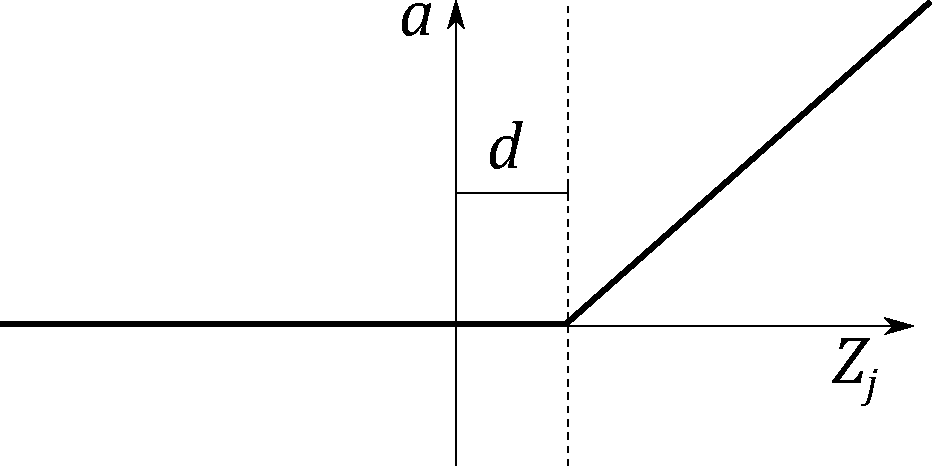
\includegraphics[width=0.5\linewidth]{images/relu.pdf}
%
%    \caption{In figure captions, explain what the reader is looking at: ``A schematic of the rectifying linear unit, where $a$ is the output amplitude,
%    $d$ is a configurable dead-zone, and $Z_j$ is the input signal'', as well as why the reader is looking at this:
%    ``It is notable that there is no activation \emph{at all} below 0, which explains our initial results.''
%    \textbf{Use vector image formats (.pdf) where possible}. Size figures appropriately, and do not make them over-large or too small to read.
%    }
%
%    % use the notation fig:name to cross reference a figure
%    \label{fig:relu}
%\end{figure}
%
%
%\begin{figure}
%    \centering
%    \begin{subfigure}[b]{0.45\textwidth}
%        
\includegraphics[width=\textwidth]{images/synthetic.png}
%        \caption{Synthetic image, black on white.}
%        \label{fig:syn1}
%    \end{subfigure}
%    ~ %add desired spacing between images, e. g. ~, \quad, \qquad, \hfill etc.
%      %(or a blank line to force the subfigure onto a new line)
%    \begin{subfigure}[b]{0.45\textwidth}
%        
\includegraphics[width=\textwidth]{images/synthetic_2.png}
%        \caption{Synthetic image, white on black.}
%        \label{fig:syn2}
%    \end{subfigure}
%    ~ %add desired spacing between images, e. g. ~, \quad, \qquad, \hfill etc.
%    %(or a blank line to force the subfigure onto a new line)
%    \caption{Synthetic test images for edge detection algorithms. \subref{fig:syn1} shows various gray levels that require an adaptive algorithm. \subref{fig:syn2}
%    shows more challenging edge detection tests that have crossing lines. Fusing these into full segments typically requires algorithms like the Hough transform.
%    This is an example of using subfigures, with \texttt{subref}s in the caption.
%    }\label{fig:synthetic}
%\end{figure}
%
%\clearpage
%
%\subsection{Equations}
%
%Equations should be typeset correctly and precisely. Make sure you get parenthesis sizing correct, and punctuate equations correctly
%(the comma is important and goes \textit{inside} the equation block). Explain any symbols used clearly if not defined earlier.
%
%For example, we might define:
%\begin{equation}
%    \hat{f}(\xi) = \frac{1}{2}\left[ \int_{-\infty}^{\infty} f(x) e^{2\pi i x \xi} \right],
%\end{equation}
%where $\hat{f}(\xi)$ is the Fourier transform of the time domain signal $f(x)$.
%
%\subsection{Algorithms}
%Algorithms can be set using \texttt{algorithm2e}, as in Algorithm \ref{alg:metropolis}.
%
%% NOTE: line ends are denoted by \; in algorithm2e
%\begin{algorithm}
%    \DontPrintSemicolon
%    \KwData{$f_X(x)$, a probability density function returing the density at $x$.\; $\sigma$ a standard deviation specifying the spread of the proposal distribution.\;
%    $x_0$, an initial starting condition.}
%    \KwResult{$s=[x_1, x_2, \dots, x_n]$, $n$ samples approximately drawn from a distribution with PDF $f_X(x)$.}
%    \Begin{
%        $s \longleftarrow []$\;
%        $p \longleftarrow f_X(x)$\;
%        $i \longleftarrow 0$\;
%        \While{$i < n$}
%        {
%            $x^\prime \longleftarrow \mathcal{N}(x, \sigma^2)$\;
%            $p^\prime \longleftarrow f_X(x^\prime)$\;
%            $a \longleftarrow \frac{p^\prime}{p}$\;
%            $r \longleftarrow U(0,1)$\;
%            \If{$r<a$}
%            {
%                $x \longleftarrow x^\prime$\;
%                $p \longleftarrow f_X(x)$\;
%                $i \longleftarrow i+1$\;
%                append $x$ to $s$\;
%            }
%        }
%    }
%
%\caption{The Metropolis-Hastings MCMC algorithm for drawing samples from arbitrary probability distributions,
%specialised for normal proposal distributions $q(x^\prime|x) = \mathcal{N}(x, \sigma^2)$. The symmetry of the normal distribution means the acceptance rule takes the simplified form.}\label{alg:metropolis}
%\end{algorithm}


\chapter{Evaluation}\label{ch:evaluation}
\section{Comparison to Sockets}\label{sec:comparison-to-sockets}
Since the aim of the API is to replace the existing BSD sockets API, a comparison between both APIs is important.
For this comparison, two implementations of a program which attempts a DNS lookup for a given domain name and connects
to first successful connection attempt, prioritising IPv6 addresses over IPv4 addresses.
See Appendix~\ref{ch:bsd-sockets-connection-code} for the sockets code and Appendix~\ref{ch:taps-connection-evaluation-code}
for the TAPS code.

\subsection{Latency Comparison}\label{subsec:latency-comparison}
Performance is important for network programming, and as discussed in Chapter~\ref{ch:analysis/requirements} the new
API should have performance similar to BSD sockets (sockets).
To have a fair comparision between the two API, the sockets version must also prioritise IPv6 addresses over IPv4
addresses, since the TAPS version does this internally.
Since a DNS lookup could have a large impact on the total latency, the domain tested is requested multiple times before
running the program under test.
See Appendix~\ref{ch:bash-script-for-latency-testing} for the script used to test the two programs.

\begin{figure}[h]
    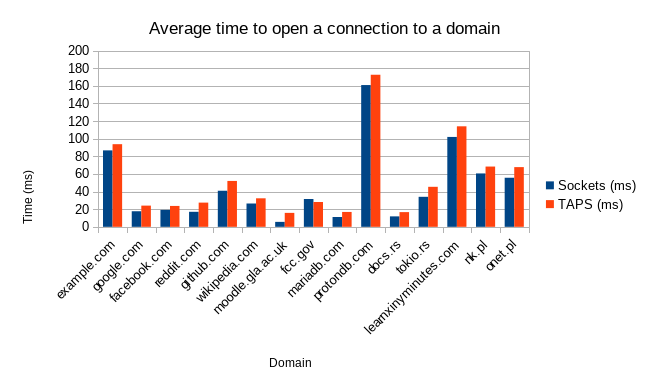
\includegraphics[width=\textwidth]{../data/avg_latency}
    \caption{A graph to show the average time over 10 attempts to connect to a range of domains.}
    \label{fig:latency}
\end{figure}

One style of network program is a short-lived program which only opens a single connection.
A program like this is useful for scripting and Unix Pipelines.
Figure~\ref{fig:latency} shows the time it takes to open a connection with both sockets and TAPS .

Figure~\ref{fig:latency} shows the TAPS version was slower for almost all domain tested when compared to the sockets
version.
Since the sockets version is single-threaded and not asynchronous, it doesn't need to set up a runtime for
\texttt{Future}s unlike the TAPS version.
In this particular test, the runtime had to be initialised ten times for each domain tested, leading to an overhead the
sockets version lacks.

\subsection{Code Comparison}\label{subsec:lines-of-code-comparison}
While lines of code is not a good metric to determine the quality of code, the substantial difference between the two
implementations is worth discussing.
Since sockets is a lower level library than TAPS, more code is required to do the same work as in TAPS .
Opening a connection with the sockets API requires the following:
\begin{itemize}
    \item DNS lookup via \texttt{getaddrinfo}
    \item Reorder DNS responses to prioritise IPv6 addresses
    \item Open a socket
    \item Connect to the remote server
\end{itemize}
The TAPS API does this all within \emph{Preconnection}'s \texttt{initiate} method.

%How good is your solution? How well did you solve the general problem, and what evidence do you have to support that?
%
%\section{Guidance}
%\begin{itemize}
%    \item
%        Ask specific questions that address the general problem.
%    \item
%        Answer them with precise evidence (graphs, numbers, statistical
%        analysis, qualitative analysis).
%    \item
%        Be fair and be scientific.
%    \item
%        The key thing is to show that you know how to evaluate your work, not
%        that your work is the most amazing product ever.
%\end{itemize}
%
%\section{Evidence}
%Make sure you present your evidence well. Use appropriate visualisations, reporting techniques and statistical analysis, as appropriate.
%
%If you visualise, follow the basic rules, as illustrated in Figure~\ref{fig:boxplot}:
%\begin{itemize}
%\item Label everything correctly (axis, title, units).
%\item Caption thoroughly.
%\item Reference in text.
%\item \textbf{Include appropriate display of uncertainty (e.g. error bars, Box plot)}
%\item Minimize clutter.
%\end{itemize}
%
%See the file \texttt{guide\_to\_visualising.pdf} for further information and guidance.
%
%\begin{figure}
%    \centering
%    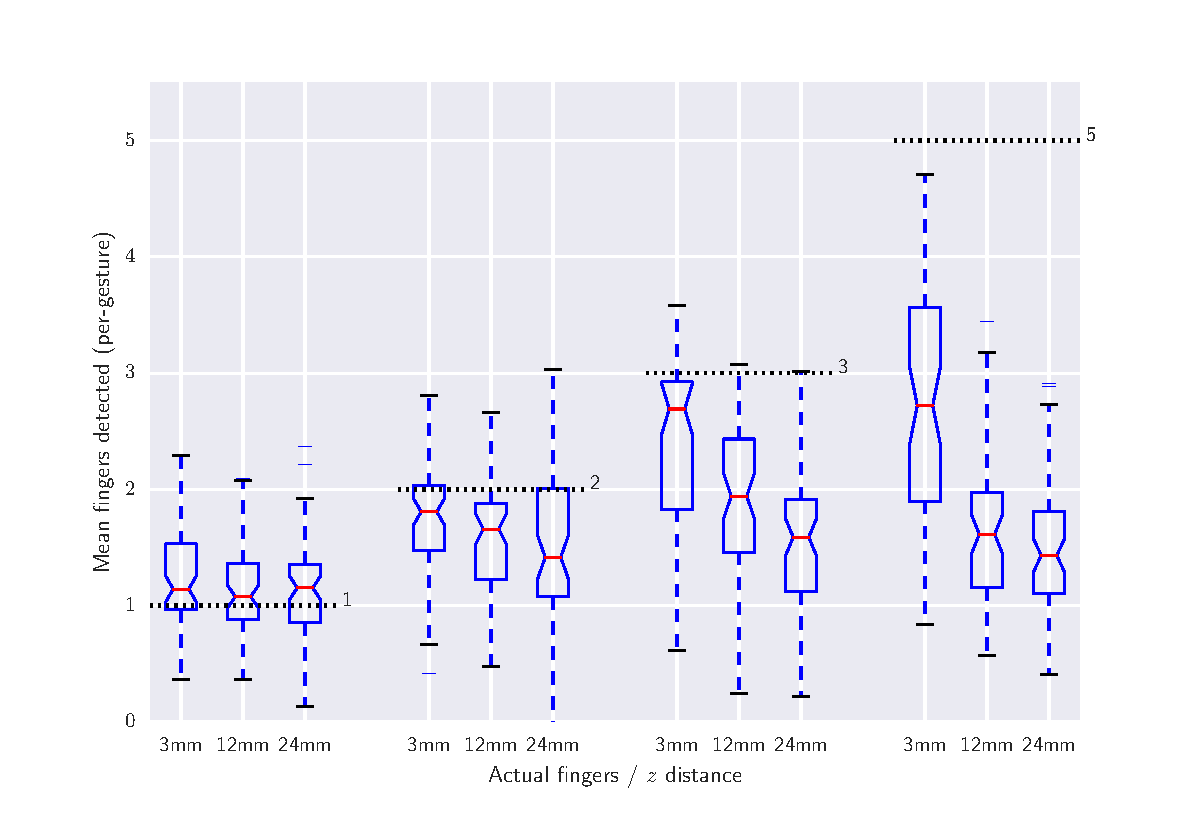
\includegraphics[width=1.0\linewidth]{images/boxplot_finger_distance.pdf}
%
%    \caption{Average number of fingers detected by the touch sensor at different heights above the surface, averaged over all gestures. Dashed lines indicate
%    the true number of fingers present. The Box plots include bootstrapped uncertainty notches for the median. It is clear that the device is biased toward
%    undercounting fingers, particularly at higher $z$ distances.
%    }
%
%    % use the notation fig:name to cross reference a figure
%    \label{fig:boxplot}
%\end{figure}


%==================================================================================================================================
\chapter{Conclusion}\label{ch:conclusion}
%Summarise the whole project for a lazy reader who didn't read the rest (e.g. a prize-awarding committee).
%\section{Guidance}
%\begin{itemize}
%    \item
%        Summarise briefly and fairly.
%    \item
%        You should be addressing the general problem you introduced in the
%        Introduction.
%    \item
%        Include summary of concrete results (``the new compiler ran 2x
%        faster'')
%    \item
%        Indicate what future work could be done, but remember: \textbf{you
%        won't get credit for things you haven't done}.
%\end{itemize}

%==================================================================================================================================
%
%
%==================================================================================================================================
%  APPENDICES

\begin{appendices}
    \chapter{Appendices}\label{ch:appendices}

%Typical inclusions in the appendices are:
%
%\begin{itemize}
%\item
%  Copies of ethics approvals (required if obtained)
%\item
%  Copies of questionnaires etc. used to gather data from subjects.
%\item
%  Extensive tables or figures that are too bulky to fit in the main body of
%  the report, particularly ones that are repetitive and summarised in the body.
%
%\item Outline of the source code (e.g. directory structure), or other architecture documentation like class diagrams.
%
%\item User manuals, and any guides to starting/running the software.
%
%\end{itemize}
%
%\textbf{Don't include your source code in the appendices}. It will be
%submitted separately.

\end{appendices}

%==================================================================================================================================
%   BIBLIOGRAPHY

% The bibliography style is abbrvnat
% The bibliography always appears last, after the appendices.

\bibliographystyle{abbrvnat}

\bibliography{l4proj}

\end{document}
